\chapter{Physics}
\label{cha:overview}

\section{Range Calculation}
\label{sec:range}

The principle of operation of an FMCW radar is shown in Fig.~\ref{fig:fmcw-principle}. A sinusoidal
signal that ramps in frequency is transmitted through air via an antenna. The reflected signal is
picked up by another antenna and mixed with the original signal.

\begin{figure}[h]
        \centering
        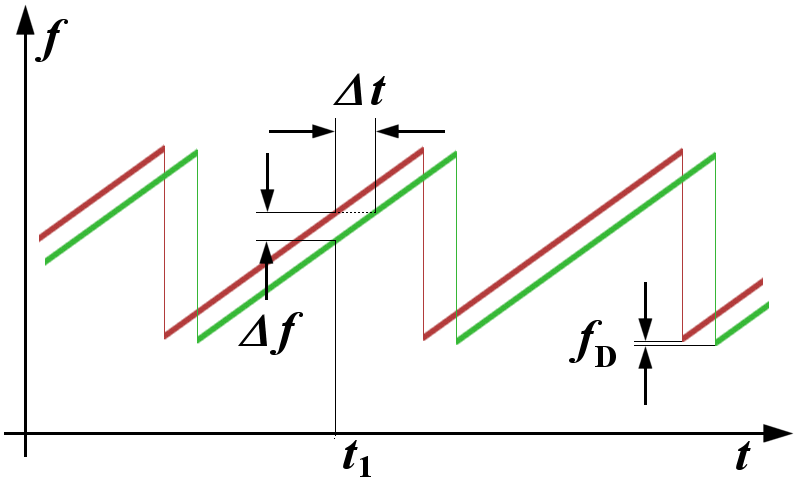
\includegraphics[width=0.75\textwidth]{data/fmcw-principle}
        \caption{FMCW radar operation: a delayed signal is modulated with the original signal and
          the distance to the remote object can be backed out from the phase difference between the
          two signals.}
        \label{fig:fmcw-principle}
\end{figure}

Because the signal travels at the speed of light, the distance to the object can be computed using
Eq.~\ref{eq:distance-generic}.

\begin{equation}
        \label{eq:distance-generic}
        d = \frac{c t_{\text{d}}}{2}
\end{equation}

$c$ is the speed of light, $t_{\text{d}}$ is the time delay and the 2 is necessary because we are
computing the round-trip time. By using the programmed frequency ramp rate we can express this
equation in terms of the frequency difference instead of the time delay\footnote{It's acceptable to
  confine ourselves to a single ramp period for each object since the max distance we can detect
  with a $1 \si{ms}$ ramp period is about $150 \si{km}$, well beyond the radar's other physical
  limits. We'll ignore the edge case where the transmitted and received signals bridge a ramp
  boundary.}. This is shown in Eq.~\ref{eq:distance-freq}.

\begin{equation}
        \label{eq:distance-freq}
        d = \frac{c t_{\text{ramp}} \Delta f}{2 f_{\text{ramp}}}
\end{equation}

Now we just need to figure out the frequency difference between the transmitted and received
signals. The transmitted signal during one ramp is:

\begin{align}
  s_{\text{t}}(t) &= T \sin\left(\omega_{\text{t}}(t) t\right)  && \text{$T$ is the transmitted
                                                                   signal's amplitude.} \\
                  &= T \sin\left(2 \pi f(t) t\right) \\
                  &= T \sin\left(2 \pi t \left( f_0 + t \frac{f_{\text{ramp}}}{t_{\text{ramp}}}
                    \right) \right)
\end{align}

The corresponding received signal is:

\begin{align}
  s_{\text{r}}(t-t_{\text{d}}) &= R \sin \left(\omega_{\text{r}}(t-t_{\text{d}})
                                 (t-t_{\text{d}})\right) \\
                               &= R \sin \left(2 \pi \left(f(t-t_{\text{d}}) +
                                 f_{\text{D}}\right)(t-t_{\text{d}})\right) && \text{$f_{\text{D}}$
                                                                               is the Doppler
                                                                               shift.}
\end{align}

The mixer computes the product of these two signals:

\begin{align}
  m &= s_{\text{t}}(t) s_{\text{r}}(t-t_{\text{d}}) \\
    &\approx T R \cos \left( \omega_{\text{t}}t - \omega_{\text{r}}t + \omega_{\text{r}}t_{\text{d}}
      \right) && \text{\footnotemark} \\
    &\approx T R \cos \left( (\omega_{\text{t}} - \omega_{\text{r}})t + \phi \right)
\end{align}
\footnotetext{We've used the identity
  $\sin\theta\sin\phi = \left[\cos(\theta - \phi) - \cos(\theta + \phi)\right]/2$ and the fact that
  the sum term is well outside the \hyperref[sec:adl5802]{mixer} output IF range (as well as the
  subsequent \hyperref[sec:ada4940-2]{IF amplifier} pass-band) and will therefore be filtered out.}

$\omega_{\text{r}}t_{\text{d}} = \phi$ is a phase term since it is not a function of $t$ and
therefore doesn't affect the frequency. So, we see that the mixer output is a signal whose frequency
is equal to the difference frequency between the transmitted and received signals. We can use the
Fourier transform to determine this frequency while ignoring the irrelevant coefficient terms and
phase shift. The Fourier transform also makes it easy to separate different objects which will each
show up as a separate frequency difference. The one complicating factor is that the received
frequency encodes the Doppler shift in addition to the distance. So, what we actually measure is
$2 \pi (\Delta f - f_{\text{D}})$ instead of $2 \pi \Delta f$. To correct for the Doppler shift we
can take multiple measurements of the object to compute its speed\footnote{The fact that the
  individual distance calculations are inaccurate by the Doppler shift doesn't matter here since the
  speed will be constant on the order of the ADC sampling period and will therefore only produce a
  constant translation that is cancelled out when computing successive displacements.} and then use
the non-relativistic equation for the Doppler shift given by Eq.~\ref{eq:doppler}.

\begin{equation}
        \label{eq:doppler}
        f_{\text{D}} = \frac{v_{\text{r}}}{c} f_0
\end{equation}

$v_{\text{r}}$ is the object's computed speed and $f_0$ is the instantaneous ramp frequency. This
must be added back in to the original result to get the true distance. However, because the speeds
we're dealing with are sufficiently low, the Doppler contribution can be effectively ignored. For
instance, the Doppler shift contribution to the distance measurement caused by a car on the highway
travelling at $70 \si{mi/h}$ is only $14 \si{cm}$. This consideration only really becomes important
when using radar for military applications such as for high-speed aircraft or missile defense.

\section{Radar Equation}
\label{sec:radar-equation}

\fixme{There's a really good description of the radar equation derivation at
  \href{http://www.radartutorial.eu/01.basics/The\%20Radar\%20Range\%20Equation.en.html}{this
    link}. It should be incorporated here to provide an intuitive understanding of this equation.}

The maximum range detectable by a radar is given by the radar equation, Eq.~\ref{eq:radar}.

\begin{equation}
        \label{eq:radar}
        R_{\text{max}} = \sqrt[4]{\frac{P_{\text{t}} G^2 \lambda^2 \sigma}{P_{\text{min}} {(4
              \pi)}^3}}
\end{equation}

\label{tab:radar-equation}
\begin{tabularx}{\textwidth}{l X l}
        \toprule
        Variable & Description & Value \\
        \midrule
        $P_{\text{t}}$ & Transmitted power. & $19.5 \si{dBm}$\footnote{$26 \si{dBm}$ adjusted for
          the 75\% \hyperref[sec:antenna-transmission]{antenna} efficiency.} \\
        $G$ & Antenna gain. & $14 \si{dBi}$ \\
        $\lambda$ & Wavelength. & $5.4 \si{cm}$\footnote{Using the center frequency, $5.6 \si{GHz}$.} \\
        $\sigma$ & Target cross section. & $1 \si{m^2}$ \\
        $P_{\text{min}}$ & Minimum detectable signal power. & $-118 \si{dBm}$\footnote{See
          \cref{sec:min-detectable-power}.} \\
        \bottomrule
\end{tabularx}

Plugging these values in, we find a maximum range of $357 \si{m}$. Using \cref{sec:range} above,
this corresponds to a maximum difference frequency of $1.4 \si{MHz}$.

In order to find the minimum range that avoids distortion, it's helpful to work backward from the
maximum \hyperref[sec:ltc2292]{ADC} differential input voltage of $2 \si{V}$. The
\hyperref[sec:ada4940-2]{IF amplifier} that feeds this input has a gain of $23 \si{dB}$ and employs
an input filter with a gain of $-10 \si{dBV}$ through most of the passband. Collectively, this
permits a \hyperref[sec:adl5802]{mixer} differential output voltage of up to $0.4 \si{V}$. As
described on Henrik's blog, we can use the equation $V = \sqrt{Z_{\text{load}} P}$ to translate this
into a output power level. Since the mixer's differential output impedance is $200 \si{\Omega}$, the
maximum acceptable output power is $-0.5 \si{dBm}$. It's power conversion gain at $5.5 \si{GHz}$ is
$-3 \si{dB}$ and the collective gain of the \hyperref[sec:sky65404]{LNA} and
\hyperref[sec:trf37a73]{RF amplifier} is $24 \si{dB}$, which sets the maximum input power at
$-21.5 \si{dBm}$. This corresponds to a distance of $1.4 \si{m}$ and difference frequency of
$5.5 \si{kHz}$. This input power is also below the IP1dB of the LNA and RF amplifier system of
$-16.5 \si{dBm}$.

\subsection{Minimum Detectable Power}
\label{sec:min-detectable-power}

In order to determine the minimum detectable power, we must find the noise power and then the SNR
that yields a readily detectable signal. Henrik's blog, as well as
\href{http://www.wireless-nets.com/resources/tutorials/define_SNR_values.html}{this site} recommend
using $20 \si{dB}$ as the minimum SNR\@. To find the noise power, we find the thermal noise and then
multiply it by the bandwidth for one FFT bin (Eq.~\ref{eq:johnson-noise}). We then add the receiver
noise figure.

\begin{equation}
        \label{eq:johnson-noise}
        P = k_{\text{B}} T B
\end{equation}

$k_{\text{B}}$ is the Boltzmann constant, $T$ is the temperature (we use $300 \si{K}$ which is often
used for room temperature) and $B$ is the bandwidth of a single FFT bin in $\si{Hz}$. A single FFT
bin bandwidth is given by Eq.~\ref{eq:fft-bin-bandwidth}.

\begin{align}
        \label{eq:fft-bin-bandwidth}
        B &= \frac{f_{\text{s}}}{N} && \text{$N$ is the number of FFT samples.} \\
        &= \frac{f_{\text{s}}}{f_{\text{s}} t_{\text{ramp}}} && \text{$t_{\text{ramp}}$ is the ramp
                                                                duration, or $1 \si{ms}$.} \\
        &= 1 \si{kHz}
\end{align}

The last step is to determine the receiver noise figure. When two components are connected together,
the equivalent noise factor is given by Eq.~\ref{eq:equiv-noise-factor}.

\begin{equation}
        \label{eq:equiv-noise-factor}
        F_{\text{NET}} = F_1 + \frac{F_2 - 1}{G_1}
\end{equation}

$F_1$ and $F_2$ are the noise factors of each component and $G_1$ is the gain of component 1. Noise
figure is the decibel equivalent of noise factor (Eq.~\ref{eq:noise-fig}).

\begin{equation}
        \label{eq:noise-fig}
        \text{NF} = 10 \log(\text{F})
\end{equation}

Eq.~\ref{eq:equiv-noise-factor} shows why it's important to have an LNA with high gain: it reduces
the noise contributions of later components. The only component whose noise figure is not listed on
its datasheet is the \hyperref[sec:ada4940-2]{IF amplifier}. Henrik uses a guess of
$10 - 20 \si{dB}$, which we will use here as well. TI has
\href{http://www.ti.com/lit/an/slyt094/slyt094.pdf}{a paper} on this which can be used if a more
precise value is needed. The datasheet also presents information on calculating noise. We use the
same $6 \si{dB}$ value that Henrik uses. \fixme{This really shouldn't just be estimated}.

Putting all these values together gives a minimum detectable power of $-118 \si{dBm}$.

\section{Angle Calculation}
\label{sec:angle}

\fixme{Complete section.}

%%% Local Variables:
%%% mode: latex
%%% TeX-master: "fmcw-radar"
%%% End:
